\chapter{Availability in the market}

\section{Type of sensor’s manufacture}
\subsection{Competition of products}
\textbf{Gas sensor} can be made for measuring of especially large flow rates and uses the calorimetric measuring principle. Available in two versions: - Standard - Heavy Duty (in the Heavy Duty version the sensor is encapsulated in stainless steel).

\textbf{Air flow sensor} provides low pressure drop in the customer’s application, highly stable null and full scale: 
\begin{itemize}
	\item Does not require recalibration in most applications.
	\item Compact package design: Occupies less space in the customer’s enclosure, potentially reducing production costs. Enclosure size may also be reduced for easier fit into space constrained applications.
	\item Low hysteresis and repeatability errors (less than $ 0.35\% $ of reading).
	\item Provides better system accuracy, enhanced response flow time of $ 6 ms $.
	\item Low power consumption: Allows for use in portable devices and battery-powered applications.
\end{itemize}

\textbf{Flow meter sensor} operates according to Faraday's law of induction. The conductive medium flowing through a pipe in a magnetic field (M) generates a voltage which is proportional to the flow velocity (v) or volumetric flow quantity. This voltage is tapped via electrodes (E) and converted in the evaluation unit. Its resistant materials mean the sensor is suitable for a multitude of media.

\section{Data sheet example}
\begin{table}[ht]
	\centering
	\caption{Typical Features of four groups of flow sensors}
	\begin{tabular}{p{0.2\linewidth}p{0.15\linewidth}p{0.15\linewidth}p{0.15\linewidth}p{0.15\linewidth}}\toprule
		\multirow{2}{*}{Speciality} & \multicolumn{4}{c}{Sensor types} \\\cmidrule{2-5}
		& Differential pressure & Electromagnetic & Coriolis flow & Ultrasonic\\\midrule
		Volumetric flow rate measurement & volume & volume & mass & volume\\
		Velocity measurement of gas / liquid & unsuitable for gas with low flow rate & unsuitable for gas flow & unsuitable for flow rate larger than $ 20m^3/min $ & unsuitable for gas flow\\
		Special / viscous flow & suitable conditions & measured & suitable conditions &  suitable conditions\\
		Liquid/gas mixture & - & suitable conditions & suitable conditions & suitable conditions\\
		Liquid condition & - & conductive & - & -\\
		Liquid of food / drink & - & measured & measured & mostly measured\\
		Installation / maintenance & easy, periodic cleaning & moderate, little maintenance & hardly maintenance & easy installation and maintenance\\
		Accuracy & $ 0.6-2\% $ measuring range & $ 0.2-1\% $ readable value & $ 0.1-0.5\% $ readable value & $ 0.35\% $ readable value; $ 2\% $ measuring range\\\bottomrule
	\end{tabular}
\end{table}

\subsection{Air/gas flow sensor}
\begin{figure}[ht]
	\centering
	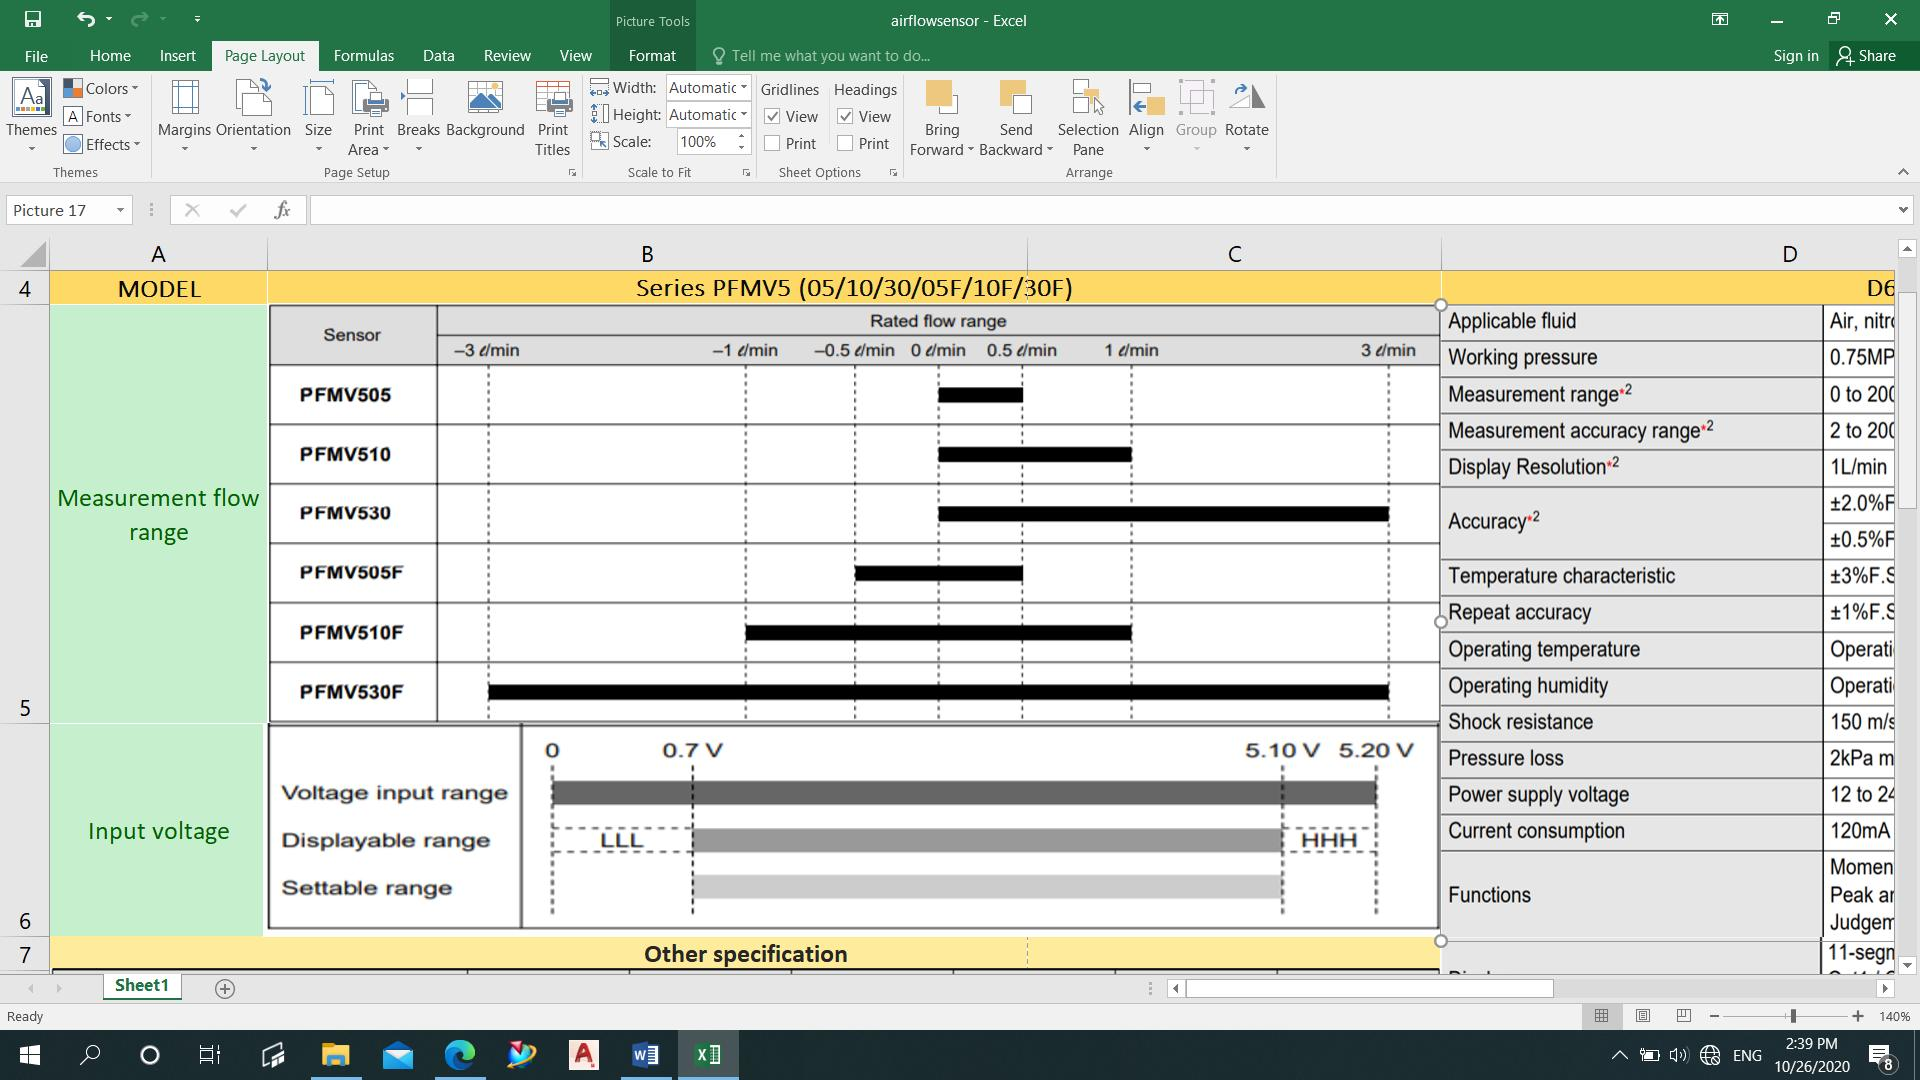
\includegraphics[width=\linewidth]{01}
\end{figure}
\clearpage

\begin{itemize}
	\item Thermal mass flow measurement.
	\item Integrated inlet and outlet pipes for flow conditioning.
	\item Pipe sizes up to $ 2'' $.
	\item Integrated display.
	\item Standard and Heavy Duty version available.
\end{itemize}
\begin{center}
	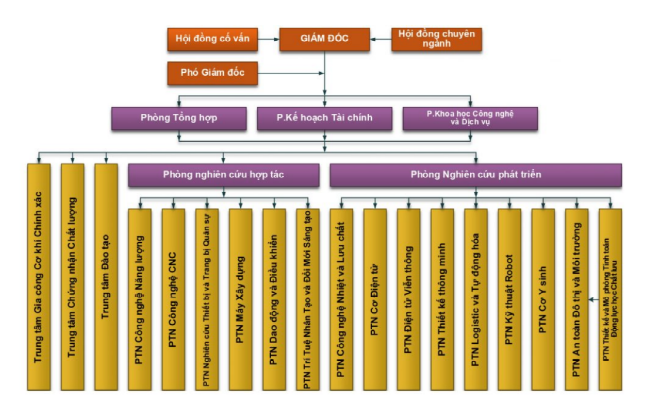
\includegraphics[width=\linewidth]{02}
\end{center}
\begin{center}
	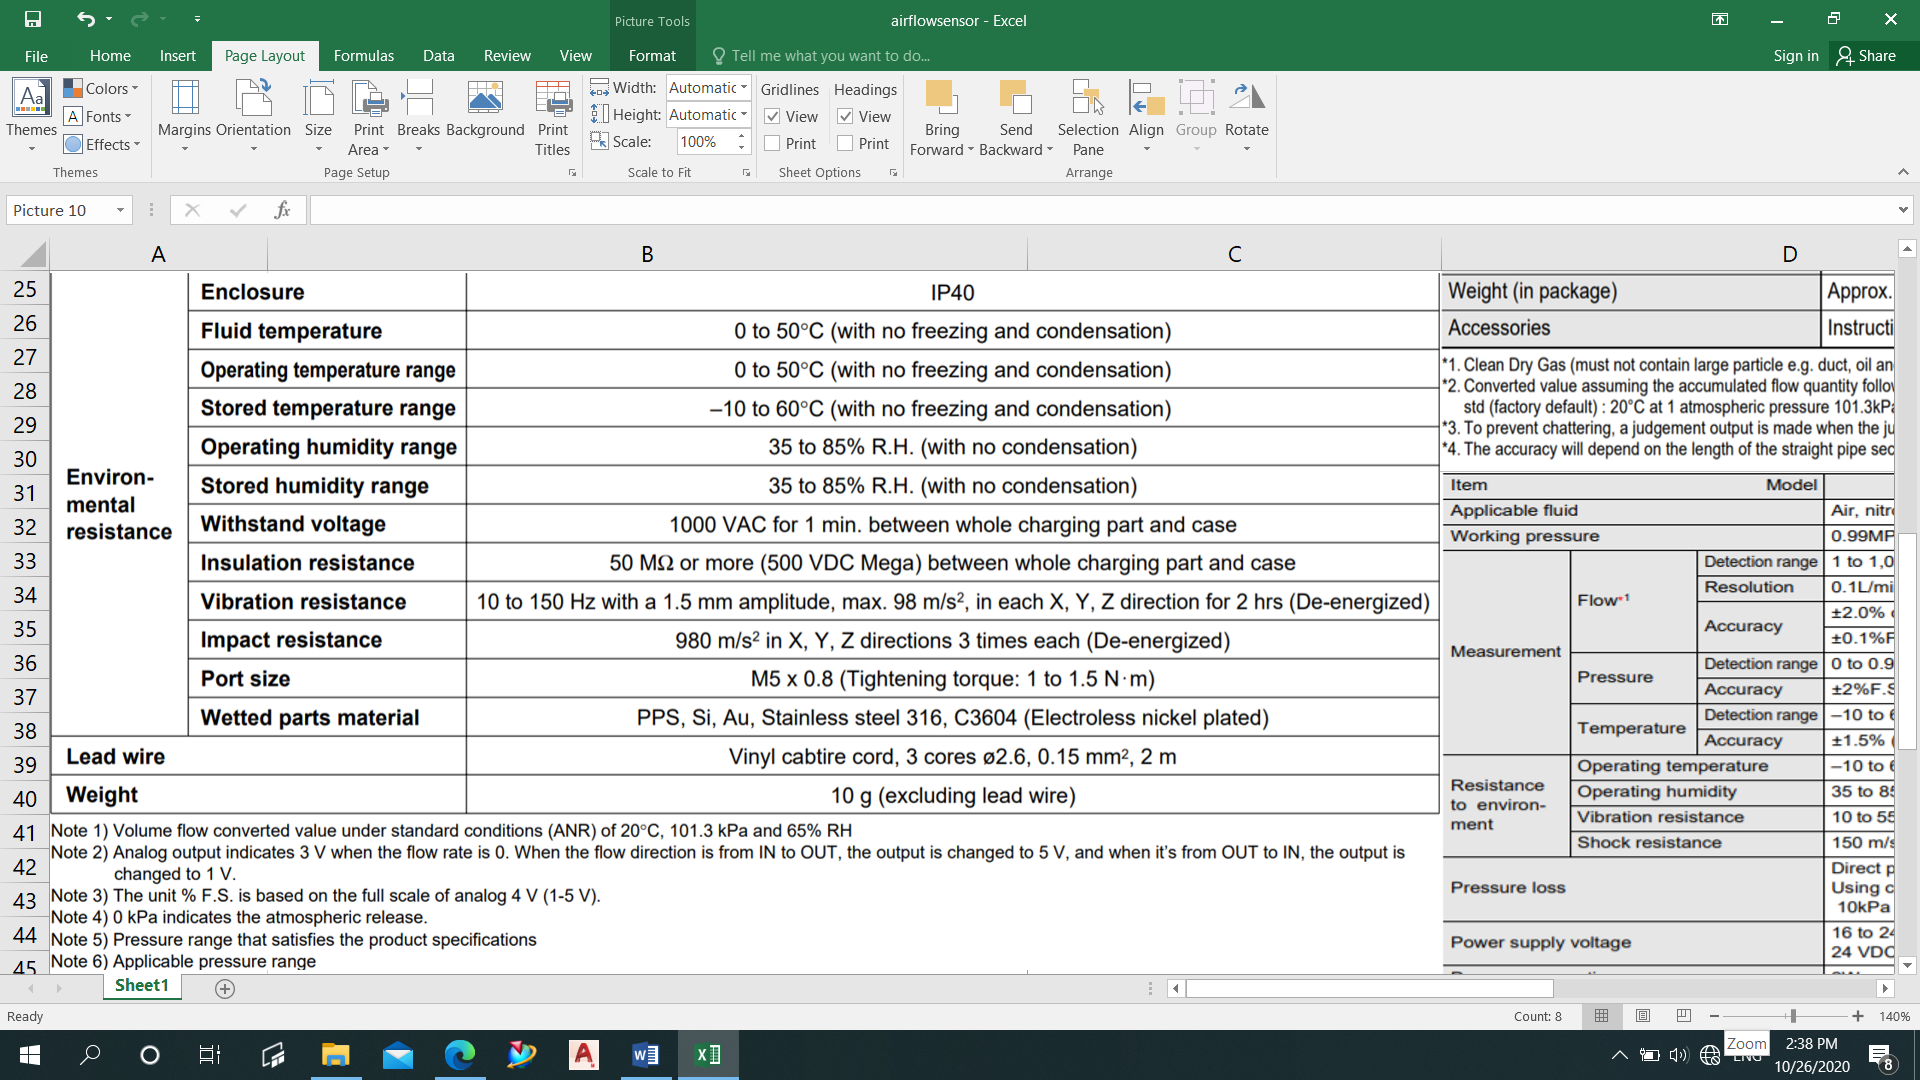
\includegraphics[width=\linewidth]{03}
\end{center}

\clearpage
\subsection{Liquid flow sensor}
\begin{center}
	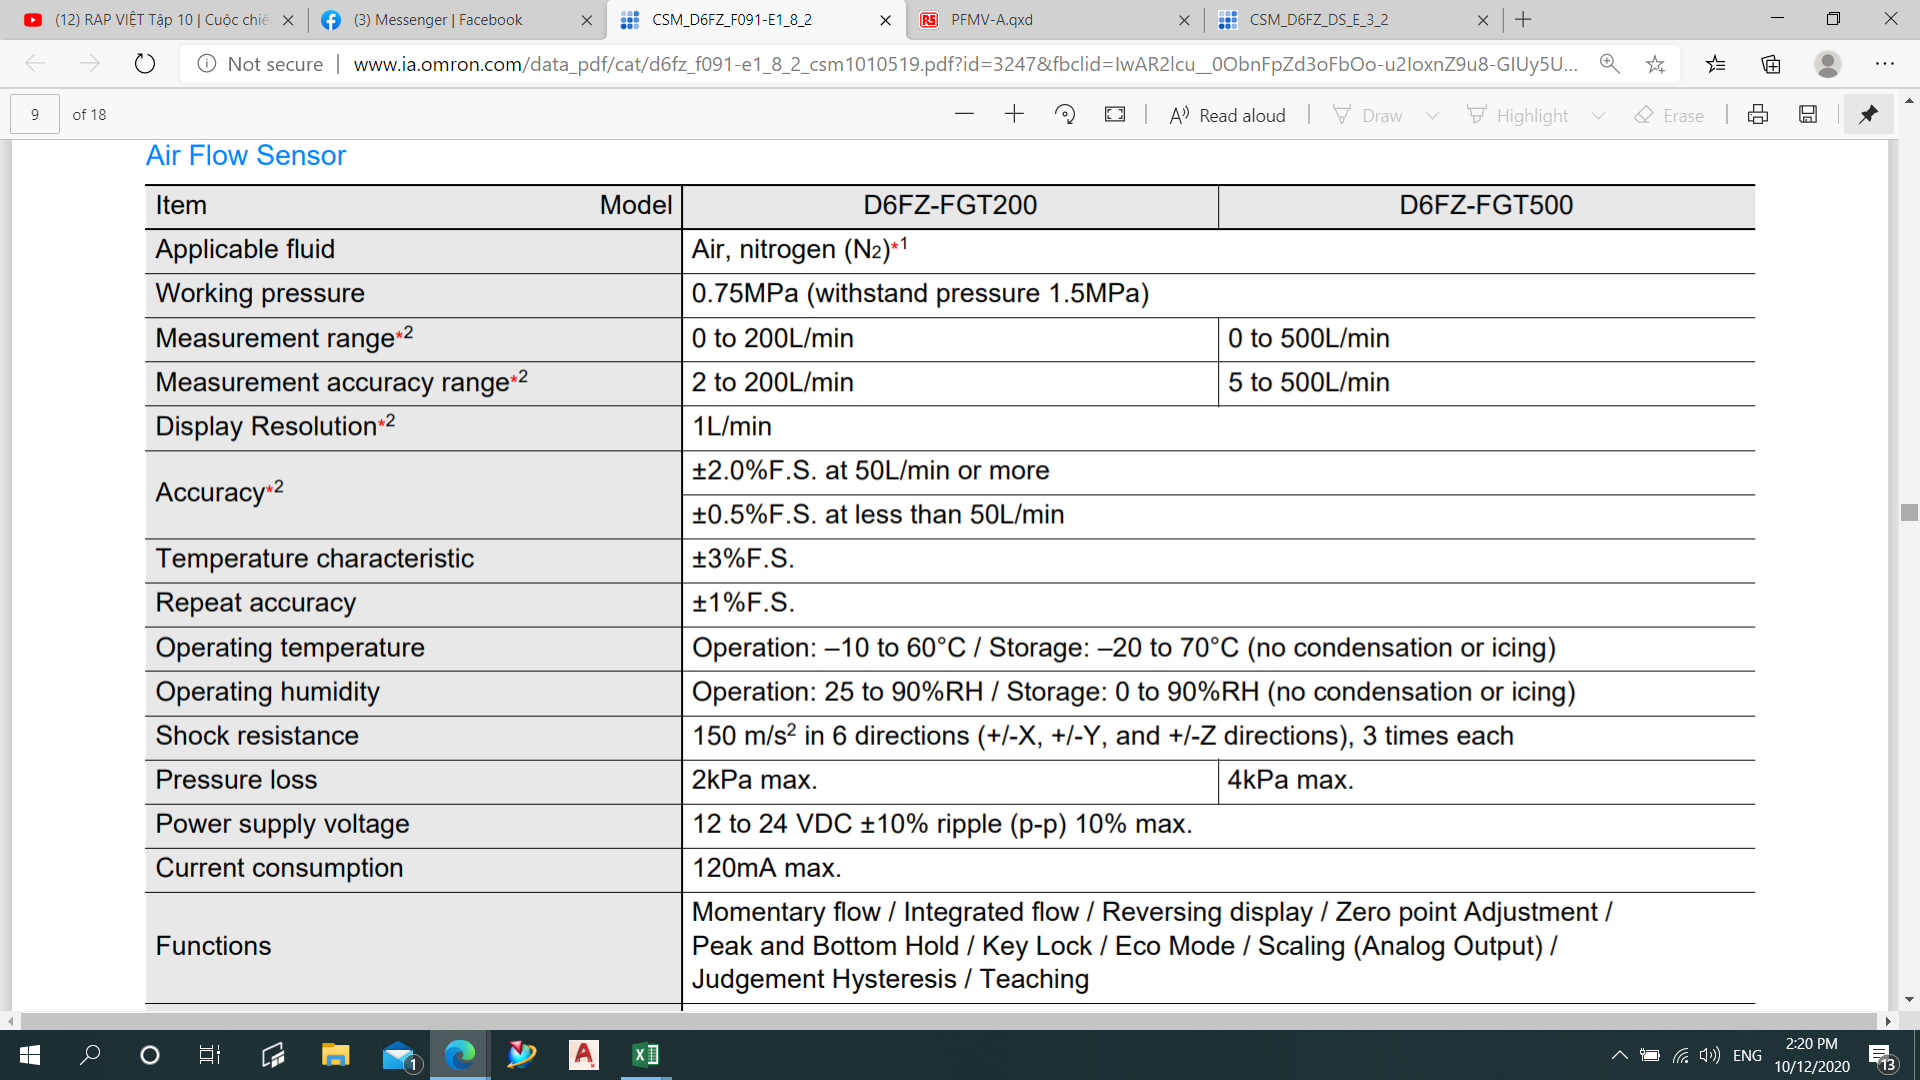
\includegraphics[width=\linewidth]{04}
\end{center}
\begin{center}
	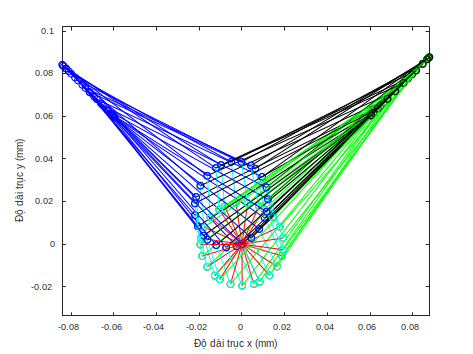
\includegraphics[width=\linewidth]{05}
\end{center}
\clearpage
\begin{center}
	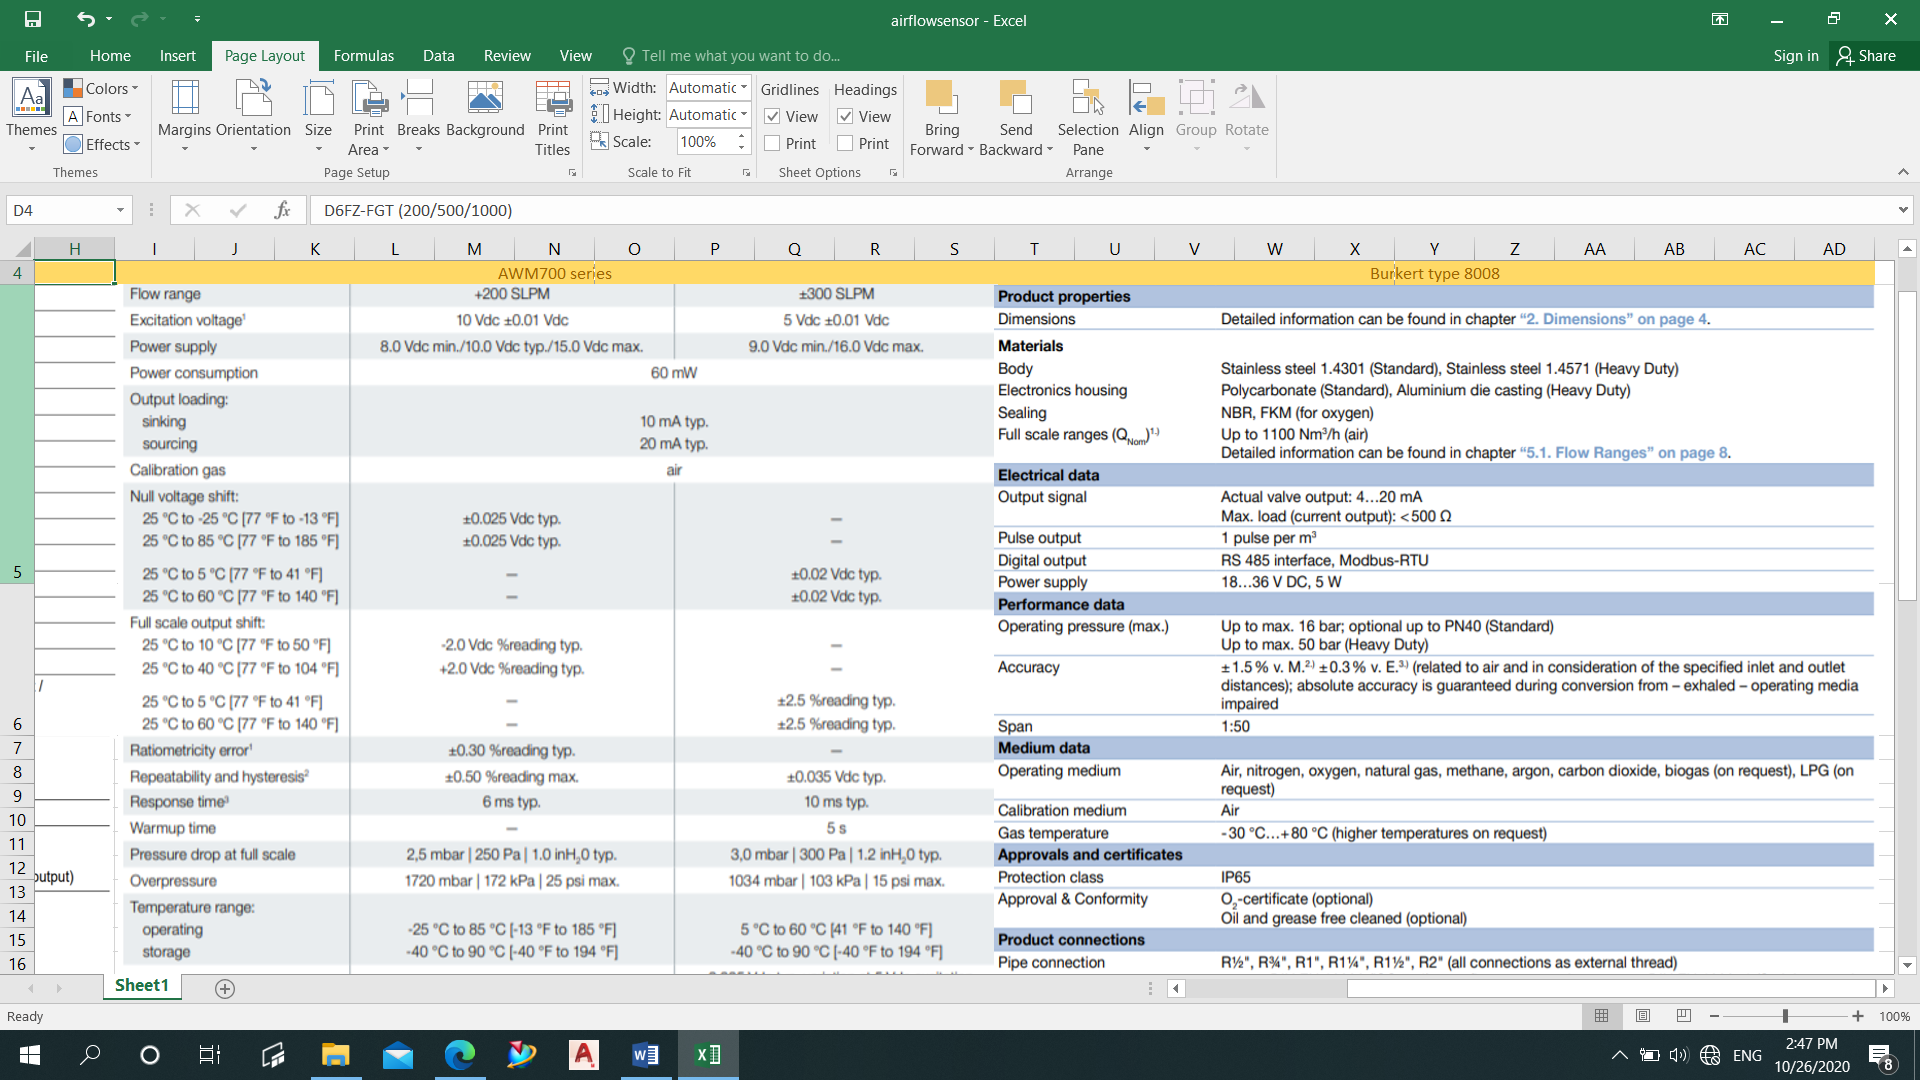
\includegraphics[width=\linewidth]{06}
\end{center}
\begin{center}
	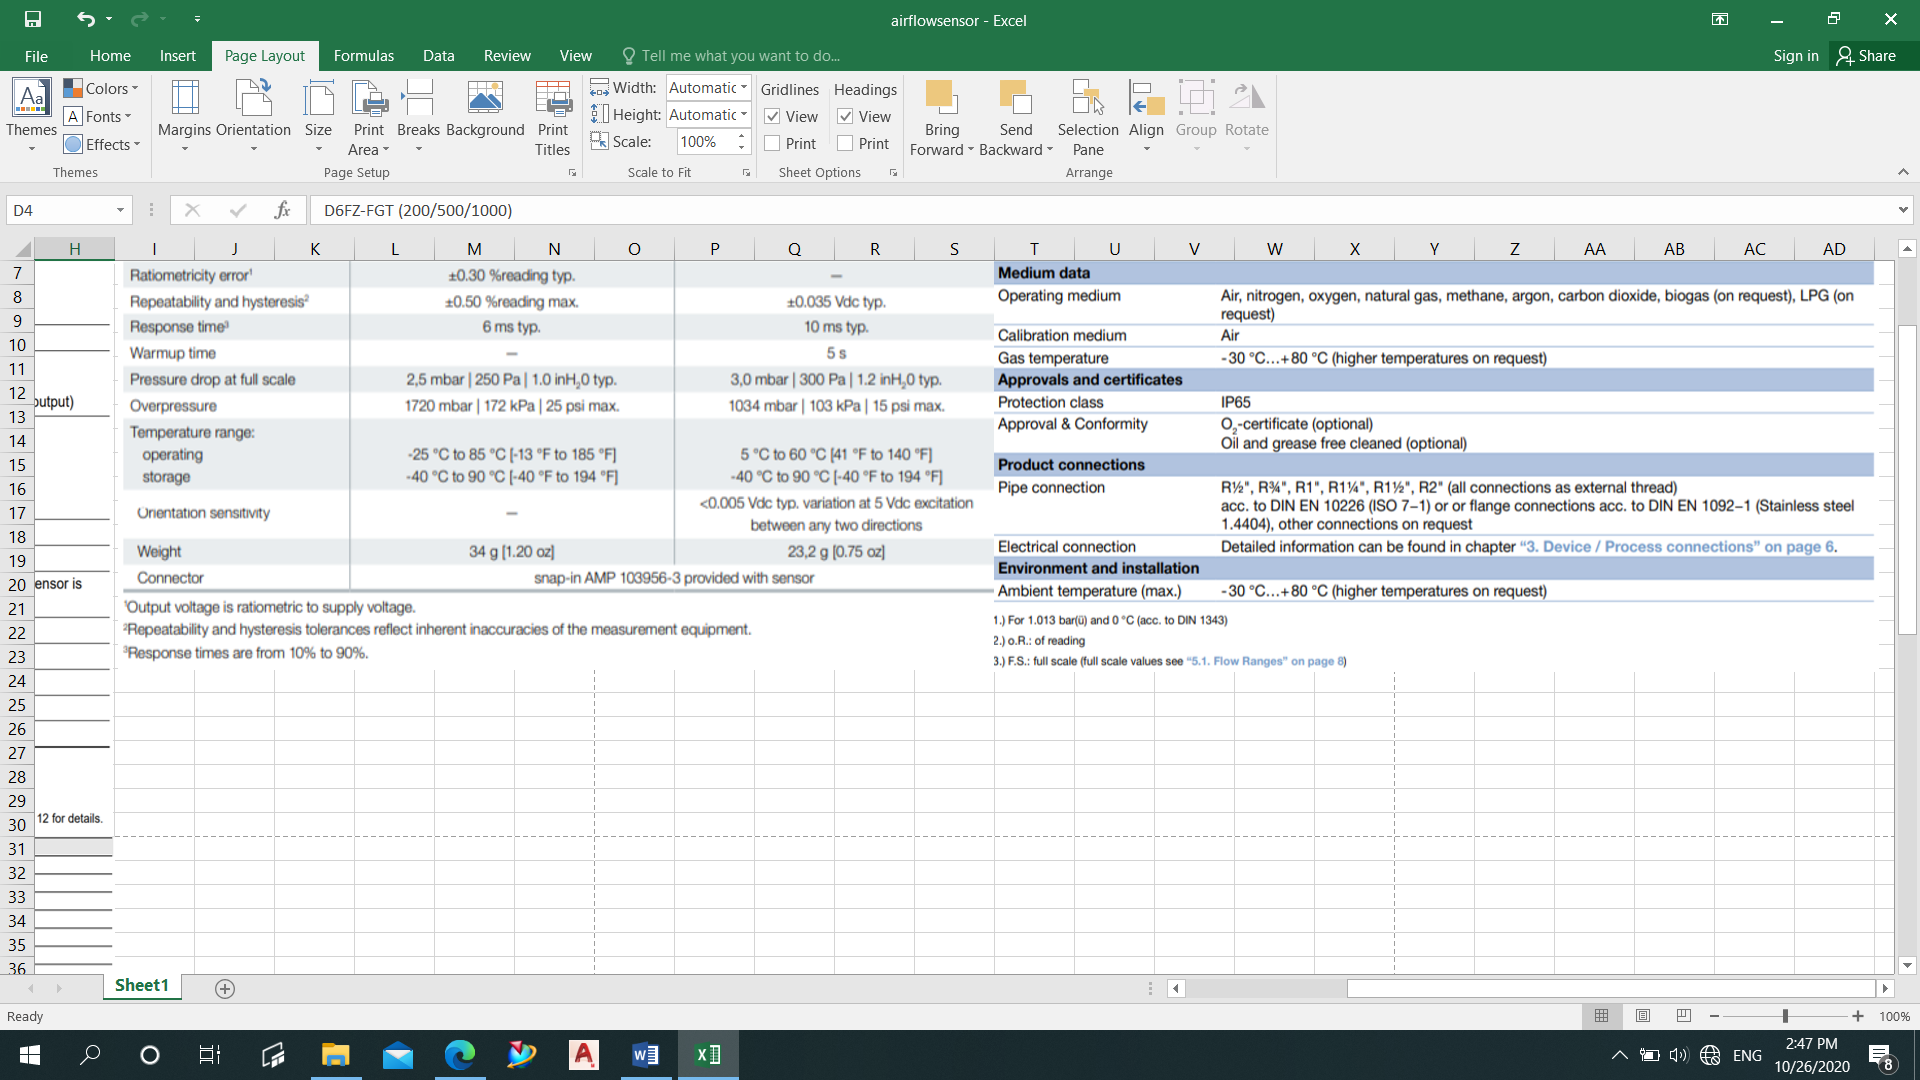
\includegraphics[width=\linewidth]{07}
\end{center}
\section{Future developments}
\subsection{Orifice Plate flowmeters for steam applications}
\paragraph{Advantages}
\begin{itemize}
	\item Simple and rugged.
	\item Good accuracy.
	\item Low cost.
	\item No calibration or recalibration is required provided calculations, tolerances and installation comply with ISO 5167.
\end{itemize}
\paragraph{Disadvantages}
\begin{itemize}
	\item Turndown is limited to between 4:1 and 5:1 because of the square root relationship between flow and pressure drop.
	\item The orifice plate can buckle due to waterhammer and can block in a system that is poorly designed or installed.
	\item The square edge of the orifice can erode over time, particularly if the steam is wet or dirty. This will alter the characteristics of the orifice, and accuracy will be affected. Regular inspection and replacement is therefore necessary to ensure reliability and accuracy.
	\item The installed length of an orifice plate flowmetering system may be substantial; a minimum of 10 upstream and 5 downstream straight unobstructed pipe diameters may be needed for accuracy.
\end{itemize}
This can include the boiler house and applicawhere steam is supplied to many plants, some on-line, some off-line, but the overall flowrate is within the range.

\subsection{Turbine flowmeters for steam applications}
\paragraph{Advantages}
\begin{itemize}
	\item A turndown of 10:1 is achievable in a good installation with the turbine bearings in good condition.
	\item Accuracy is reasonable ($ \pm 0.5\% $ of actual value).
	\item Bypass flowmeters are relatively low cost.
\end{itemize}
\paragraph{Disadvantages}
\begin{itemize}
	\item Generally calibrated for a specific line pressure. Any steam pressure variations will lead to inaccuracies in readout unless a density compensation package is included.
	\item Flow straighteners are essential (see Tutorial 4.5).
	\item If the flow oscillates, the turbine will tend to over or under run, leading to inaccuracies due to lag time.
	\item Wet steam can damage the turbine wheel and affect accuracy.
	\item Low flowrates can be lost because there is insufficient energy to turn the turbine wheel.
	\item Viscosity sensitive: if the viscosity of the fluid increases, the response at low flowrates deteriorates giving a non-linear relationship between flow and rotational speed. Software may be available to reduce this effect.
	\item The fluid must be very clean.
\end{itemize}
\paragraph{Typical Applications}
\begin{itemize}
	\item Superheated steam.
	\item Liquid flowmetering, particularly fluids with lubricating properties. As with all liquids, care must be taken to remove air and gases prior to them being metered.
\end{itemize}

\subsection{Variable Area flowmeters for steam applications}
\paragraph{Advantages}
\begin{itemize}
	\item Linear output.
	\item Turndown is approximately 10:1.
	\item Simple and robust.
	\item Pressure drop is minimal and fairly constant.
\end{itemize}
\paragraph{Disadvantages}
\begin{itemize}
	\item The tube must be mounted vertically.
	\item Because readings are usually taken visually, and the float tends to move about, accuracy is only moderate. This is made worst by parallax error at higher flowrates, because the float is some distance away from the scale.
	\item Transparent taper tubes limit pressure and temperature.
\end{itemize}
\paragraph{Typical Applications}
\begin{itemize}
	\item Metering of gases.
	\item Small bore airflow metering - In these applications, the tube is manufactured from glass, with calibrations marked on the outside. Readings are taken visually.
	\item Laboratory applications.
	\item Rotameters are sometimes used as a flow indicating device rather than a flow measuring device.
\end{itemize}